\subsection{Completed exploratory comparisons}
Effects use the equally weighted geometry means defined in
Equation~\eqref{eq:geometry-effect}. Table~\ref{tab:exploratory-complete}
reports completed comparisons with their original denominators. Positive
effects indicate lower candidate cost; repetitions within a geometry were
not treated as independent benchmark instances.

\begin{table}[htbp]
\centering
\small
\begin{tabular}{lrrr}
\toprule
Study & Runs & Reduction (\%) & W/L/T \\
\midrule
Charged TRAIN, 60 s & 54 & 1.886 & 8/1/0 \\
Conditional fixed-support replay & 27 & 2.014 & 9/0/0 \\
Limited validation, 60 s & 70 & 0.907 & 2/1/4 \\
Conditional joint insertion vs. greedy & 324 & -0.181 & 3/6/0 \\
\bottomrule
\end{tabular}
\caption{Completed exploratory comparisons. Positive reduction favors the hybrid in the first three rows and nearest-gap joint insertion in the last. W/L/T counts geometry means. Conditional rows exclude generation of their common starting states and are not directly comparable with charged end-to-end rows.}
\label{tab:exploratory-complete}
\end{table}


The corrected 60-second training experiment comprised nine geometries,
three seeds and two methods, for 54 executions. The hybrid reduced mean
cost in eight geometry means and increased it in one, with an equally
weighted reduction of 1.886\%. Independent audits checked 334 routes,
including intermediate incumbents. These observations followed several
exploratory attempts and were not a confirmatory test of generalization.

In a conditional replay, fixed-support LKH received the remaining allowance
from each of the 27 saved MDM initialization states. The hybrid had a lower
seed-mean cost in all nine geometry groups, with a mean reduction of 2.014\%
relative to this control. The replay reused training starts and excluded
their generation cost. It supplied a component comparison rather than an
independent end-to-end replication or evidence for each destruction and
repair decision separately.

Figure~\ref{fig:training-effects} displays the geometry-level heterogeneity
behind the two training averages. The largest end-to-end reduction occurred
on rd400, whereas kroA200 and ts225 showed small mean changes and tsp225
showed a small deterioration. Individual seed effects also varied within
geometries. The markers are paired observations, not uncertainty intervals;
the two panels use different controls and cannot be combined into one effect.

\begin{figure}[tbp]
\centering
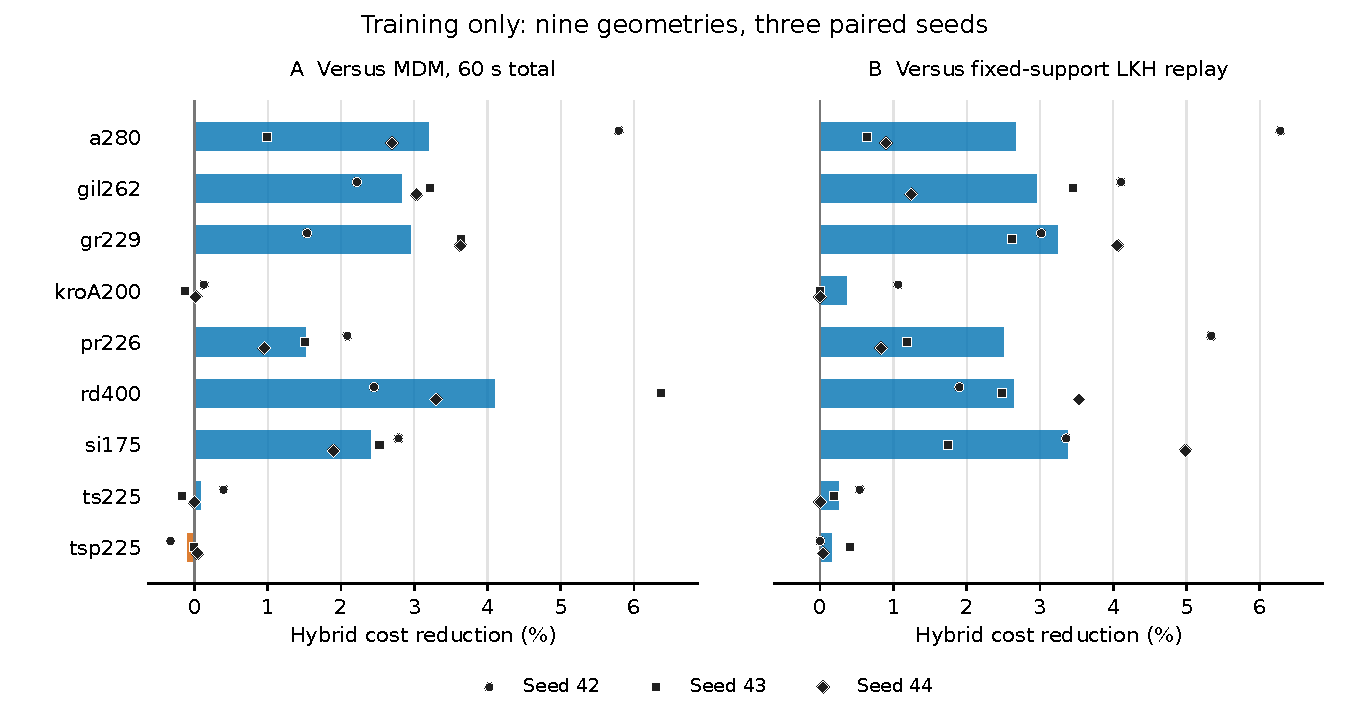
\includegraphics[width=\textwidth]{figures/hybrid_training_effects.pdf}
\caption{Completed exploratory training comparisons on nine geometries with
three paired seeds. Bars show the relative reduction of seed-mean costs;
markers show individual seed-pair reductions, not confidence intervals.
Panel A compares fresh executions with MDM under a total 60-second budget,
including initialization. Panel B uses a conditional fixed-support LKH replay
from saved initialization states and excludes their generation cost.
Positive values favor the hybrid. Neither panel provides independent test
confirmation.}
\label{fig:training-effects}
\end{figure}

The frozen validation configuration was evaluated on seven geometries with
five seeds per method, yielding 70 executions. Audits checked 466 routes
without missing runs or feasibility failures. The primary mean reduction
was 0.907\%, comprising two positive geometry means, four ties and one
negative mean. The reductions on pr264 and pr299 were 2.730\% and 3.771\%,
respectively; d198 increased by 0.150\%. The prespecified screen required
at least three positive geometry means, so the candidate did not pass.
The twelve reserved test geometries remained unopened. These validation
geometries had already been used for an earlier, different LKH configuration;
the present screen therefore did not constitute untouched confirmation.

A separate conditional training experiment compared greedy repair with
joint insertion MIP repair after matched destructions. Across 324 executions,
nearest-gap MIP repair had a mean reduction of $-0.181\%$ relative to greedy
repair and failed its prespecified mean-improvement screen. It improved on
the equal-size random-gap MIP control in eight geometry means. All 1,296
audited routes were feasible, including retained fallback incumbents; this
does not imply that every restricted repair model was feasible. The
experiment excluded generation of common MDM starts and did not establish
an end-to-end advantage for MIP integration.

Earlier clock-collector experiments are retained as separate negative
records. Their wrapper could discard an improvement observed before the
deadline when cleanup returned late. The corrected collection used absolute
incumbent event times and fresh executions; its differences from the earlier
collection cannot be attributed solely to re-extracting identical trajectories.
No result in this subsection establishes a new best-known solution, a
literature-wide novelty claim or inferential significance after exploratory
method selection. The completed longer-horizon screen is reported separately
in Section~\ref{sec:awake300-results} and is excluded from this table.
